\chapter{\acf{PaTAS}}
\label{chap:ovl}
The previous chapters established the conceptual and methodological foundations for trust assessment in general and particularly in \ac{ML} systems. In particular, \cref{chap:Trust_method} introduced a general evidence-based methodology for trust evaluation, while \cref{chap:tnasl} improved the graph-based reasoning mechanisms required to compute trust expressions. Building on these foundations, this chapter introduces the \emph{\acf{PaTAS}}, a system architecture designed to operationalize the proposed methodology in \ac{ML} pipelines. \ac{PaTAS} provides a scalable and modular framework for performing trust assessment throughout both training and inference, starting from the training dataset. The system enables the evaluation of \ac{NN} outputs in parallel with their inference by allowing different trust sources and reasoning components to be processed independently, without impacting the standard \ac{NN} inference process. This design allows efficient evaluation of trust in complex \ac{NN} systems where multiple evidence streams must be combined. The concepts presented in this chapter build upon previous publication. In particular, the architecture and core reasoning principles are derived from the work presented in~\cite{patas}, currently under review at the \emph{Elsevier Knowledge Based Systems}.

\section{Introduction}

The analysis presented in the Related Work \cref{sec:gap_summary} highlights a fundamental limitation in existing approaches to uncertainty and trust in \ac{NN} systems. While a wide range of methods have been proposed to quantify uncertainty at different levels, no unified framework simultaneously provides (i) an explicit, evidence-based representation of trust, (ii) the assessment of dataset trustworthiness during training, and (iii) a consistent propagation of trust from data to model parameters and from inputs to predictions.

Classical probabilistic and Bayesian approaches offer rigorous tools for modeling uncertainty, but they do not represent trust as a structured and composable construct. Conversely, \ac{SL} provides a principled calculus for reasoning about belief, disbelief, and uncertainty, as well as mechanisms for trust transitivity and source credibility. However, its application to \ac{NN} systems remains limited, both in terms of pipeline integration and computational realization. In particular, existing approaches do not provide a framework capable of integrating heterogeneous trust sources and propagating trust consistently across the different stages of the learning pipeline.

Furthermore, current uncertainty-aware \ac{NN} methods are typically confined to specific levels of abstraction. Model-based approaches, such as \acp{BNN}~\cite{neal1996bayesian} and deep ensembles~\cite{https://doi.org/10.1002/widm.1249}, capture parameter uncertainty but do not account for dataset credibility. Input-level propagation methods model observation uncertainty at inference time, yet they do not incorporate the reliability of the training dataset.

Existing trust-oriented approaches remain similarly limited in scope. For instance, DeepTrust~\cite{10.3389/frai.2020.00054} proposes a mechanism to leverage training dataset trustworthiness to assess model-level trust. However, such approaches are restricted to the training phase and do not extend to inference-time trust assessment, where predictions must be evaluated on a per-input basis.

To address these limitations, this chapter introduces the \emph{\acf{PaTAS}}, a system architecture designed to operationalize a unified trust assessment framework across the entire pipeline. \ac{PaTAS} enables the integration of multiple trust sources, including dataset reliability, model parameters, and input uncertainty, into a coherent and composable evaluation process.

A key feature of \ac{PaTAS} is its ability to perform trust assessment in parallel with standard \ac{NN} computations. By decoupling trust reasoning from the prediction process, the system allows trust to be computed alongside model outputs without modifying the internal structure of the \ac{NN}. This design ensures scalability, modularity, and compatibility with existing \ac{ML} systems.

This chapter focuses on the architectural design of \ac{PaTAS}, including its core components and its integration within \ac{ML} pipelines. The technical mechanisms underlying trust propagation and computation are presented in the following chapter.




\section{\ac{PaTAS} General Description}

\ac{PaTAS} is a framework designed to assess and propagate trust throughout the pipeline of a \ac{NN}. It operates in parallel with the standard neural architecture and maintains a corresponding trust flow that mirrors the \ac{ML} pipeline. This design enables trust to be evaluated continuously, from the construction of the training dataset to inference-time predictions.

The trust of the \ac{NN} output computed by \ac{PaTAS} is derived from two complementary sources:
\begin{enumerate}
    \item \textbf{Trust in model parameters}, obtained from the trustworthiness of the training dataset. This includes both the reliability of input features and the credibility of labels used during training.
    \item \textbf{Trust in inference inputs}, corresponding to the reliability of the input features provided at prediction time.
\end{enumerate}

By combining these two sources, \ac{PaTAS} enables the computation of trust in model outputs. This is particularly important as a reliable input does not necessarily guarantee a reliable prediction. For instance, an input \(x\) may be accurate and trustworthy (i.e., high trust score \(T_x\)), while the corresponding prediction \(y'\) may still be unreliable due to biased, noisy, or poorly calibrated model parameters \(\theta\) (i.e., low trust score \(T_{y'}\)). \ac{PaTAS} explicitly captures this distinction by evaluating trust across all stages of the pipeline.

Importantly, the notion of trust considered in \ac{PaTAS} is \emph{property-dependent}. Trust is always defined with respect to a specific property of interest, such as accuracy, bias, fairness, or any user-defined criterion. The assessment performed at the data level determines the nature of the trust that is propagated throughout the system. For instance, if the training dataset is evaluated with respect to accuracy, the resulting trust reflects the confidence in the correctness of predictions. Similarly, if the assessment targets bias or representativeness, the propagated trust captures the reliability of the model with respect to these properties. As a result, \ac{PaTAS} provides a flexible framework in which different trust dimensions can be analyzed independently or jointly, depending on the property under consideration.

A key design principle of \ac{PaTAS} is that it operates externally to the \ac{NN}. Rather than modifying the internal computations of the model, \ac{PaTAS} performs trust reasoning alongside the standard forward and backward passes. This non-intrusive approach preserves the original predictive behavior of the \ac{NN}, avoids additional computational overhead within the model, and ensures compatibility with existing architectures.

\marginpar{Workflow Overview}
The overall workflow of \ac{PaTAS} is illustrated in \cref{fig:ovvwptas}. The process begins at the data level, where multiple data providers contribute to a data warehouse. The collected data undergoes preprocessing steps, including data cleaning, labeling and more, resulting in the construction of the training dataset.

\ac{PaTAS} first performs a \emph{training dataset trustworthiness assessment}, where evidence from the dataset is used to quantify the reliability of both input features and labels. This step produces trust scores associated with the training data, which are then used to derive trust in the model parameters during the training process.

Once the model is trained, \ac{PaTAS} enables \emph{trust propagation within the \ac{NN}}. During inference, the system receives a query from the user, which is processed by the \ac{NN} to generate a prediction. In parallel, \ac{PaTAS} evaluates the trustworthiness of the input and propagates it through the model, combining it with parameter trust to produce a trust score associated with the output.

Importantly, this trust computation is performed as a parallel function that does not interfere with the \ac{NN} inference. As shown in \cref{fig:ovvwptas}, the system produces both a prediction and an associated trust score, enabling the user to assess not only what the model predicts, but also how reliable that prediction is.

\begin{figure}
    \centering
    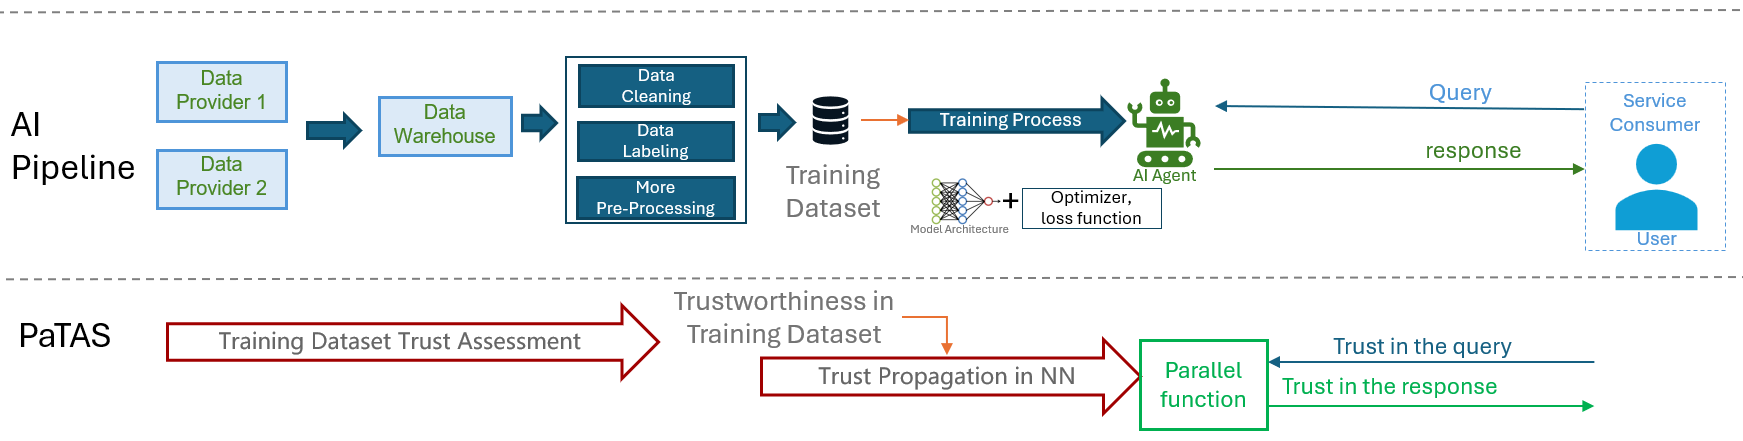
\includegraphics[width=\linewidth]{img/patas/overviewPTAS.png}
    \caption{PaTAS workflow - from dataset trustworthiness assessment to trust propagation during inference.}
    \label{fig:ovvwptas}
\end{figure}

\section{Functionalities}

\begin{figure}
    \centering
    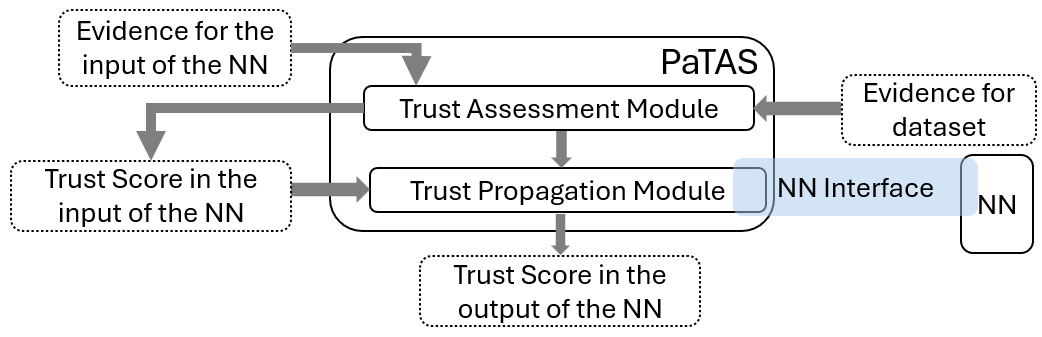
\includegraphics[width=\linewidth]{img/patas/end_to_end.png}
    \caption{Overview of the \acs{PaTAS} framework for end-to-end trust assessment in \ac{NN} pipelines.}
    \label{fig:patas_all}
\end{figure}

\subsection{Core Components}

The functionalities of \ac{PaTAS} are organized around two complementary components, as illustrated in \cref{fig:patas_all}. These components correspond to two fundamental aspects of trust assessment in \ac{ML} pipelines: (1) the evaluation of data trustworthiness, including both training datasets and input data at inference time, and (2) the propagation of trust through the \ac{NN}.

\paragraph{Trust Assessment Module} The first component focuses on the assessment of the trustworthiness of the training dataset and the input of the \ac{NN}. This assessment is \emph{property-dependent}, meaning that trust is quantified with respect to a specific property of interest, such as accuracy or bias. It relies on evidence extracted from the data, including the reliability of input features and the credibility of labels, in relation to the selected property. This process produces trust scores associated with the training samples (and input data in general), which are then used to derive trust in the learned model parameters. Consequently, the nature of the propagated trust directly depends on the property used during the assessment stage. This component establishes the foundation of trust for the entire pipeline.

\paragraph{Trust Propagation Module}
The second component is responsible for propagating trust through the \ac{NN}. It leverages the trust derived from the training dataset to assess the reliability of model parameters and combines it with the trust associated with input features at inference time. This component enables the computation of trust scores at different levels of abstraction, including neuron-level, layer-level, and output-level trust. Together, these two components form a unified framework for end-to-end trust assessment.

\subsection{Operational Phases}

The behavior of \ac{PaTAS} can be described through three operational phases, corresponding to different stages of the \ac{NN} lifecycle.
\begin{enumerate}
    \item \textbf{Dataset Trust Assessment Phase:} In the first phase, \ac{PaTAS} evaluates the trustworthiness of the training dataset. This involves analyzing the quality of input features and labels to produce trust scores associated with the training data. These scores serve as the initial source of trust for subsequent stages.
    \item \textbf{Training Propagation Phase:} In the second phase, the trust derived from the training dataset is propagated through the \ac{NN} during the training process. This phase enables the estimation of trust in the learned model parameters, reflecting how the quality of the data influences the reliability of the model.
    \item \textbf{Inference Propagation Phase:} In the third phase, \ac{PaTAS} operates during inference to assess the trustworthiness of individual predictions. Trust associated with the input is propagated through the network and combined with parameter trust to produce a trust score for the output. This enables per-instance trust evaluation and supports informed decision-making based on both predictions and their associated reliability.
\end{enumerate}

Notably, the last two phases correspond to trust propagation mechanisms, while the first phase provides the foundational trust assessment derived from the training dataset.

\section{Summary \& Conclusions}

This chapter introduced \ac{PaTAS}, a modular and scalable framework designed to operationalize trust assessment in \ac{ML} pipelines.

Building upon the general trust assessment methodology and the graph-based reasoning mechanisms presented in previous chapters, the two main components of \ac{PaTAS} provide a practical system for evaluating and propagating trust throughout both training and inference.

The framework is structured around two main components: the assessment of data trustworthiness and the propagation of trust through the \ac{NN}. These components enable the integration of multiple trust sources, including data reliability, label credibility, and input uncertainty, into a unified and composable trust evaluation process. By operating in parallel with the \ac{NN}, \ac{PaTAS} ensures that trust assessment remains non-intrusive and does not interfere with the model’s predictive behavior.

Furthermore, the definition of distinct operational phases allows \ac{PaTAS} to capture the dynamic nature of trust across the learning lifecycle, from dataset construction to inference-time prediction. This enables both global and per-instance trust evaluation, addressing key limitations of existing approaches that are confined to isolated stages or specific types of uncertainty.

Overall, \ac{PaTAS} constitutes the operational layer of the proposed trust assessment framework, bridging the gap between theoretical trust modeling and practical AI system deployment. The next chapter builds upon this architecture by formalizing the mechanisms underlying trust propagation within \acp{NN}, including the operators and computational processes that enable consistent and scalable trust reasoning.